The planning module is divided in three different parts.

\begin{enumerate}
    \item The first thing to do is to find a goal point, that goal point must be chosen in a way that will make the robot explore unknown parts of the environment.
    \item Then we have to build a path for the robot to follow between the actual position of the robot and the target.
    \item The final thing to do is to use a path tracking algorithm that will make the robot follow the built path.
\end{enumerate}

\section{Find a goal point}

In order to find a goal point we have to detect an unexplored zone that we can access to, to do so we used an approach based on frontier detection.
A frontier is a region on the border between an explored zone and an unexplored zone.
Then the first thing to do in order to determine the next goal point is to detect the frontiers.

\subsection{Detect the frontiers}

To detect the frontiers we go through all the unexplored cells of the grid and if that cell has an explored empty cell in its Von Neumann neighbourhood we know it is part of a frontier.
The Von Neumann neighbourhood is composed of the four adjacent cells around a cell.
Once we went through the whole grid we have a list of all the cells that are on a frontier, the next step is to divide them into several regions.

To divide the frontiers in regions we go through the previously built list, each time we put a cell in its region we delete it from the initial list.
For each cell we go through its Moore neighbourhood (The entire 8 cells neighbourhood).
If one of its neighbour is in the initial list we recursively call the same function.

This is the pseudocode of the 'get\_divided\_frontiers' function:

\FloatBarrier
\begin{algorithm}
    \caption{get divided frontiers}
    \label{get divided frontiers}
    \begin{algorithmic}[1]
        \Procedure{get\_frontiers}{$map$}
            \State $frontiers$ is an empty array
            \For{$cell$ \textbf{in} $map$}
                \If{$is\_unknown(cell)$}
                    \For{$neighbour$ \textbf{in} $von\_neumann\_neighbourhood(cell)$}
                        \If{$neighbour$ \textbf{not in} $frontiers$ \textbf{and} $is\_empty(neighbour)$}
                            \State $frontiers.append(neighbour)$
                        \EndIf
                    \EndFor
                \EndIf
            \EndFor
            \State \textbf{return} $frontiers$
        \EndProcedure
        \Procedure{build\_frontiers}{$frontiers,$ $current\_frontier,$ $cell$}
            \State $neighbours \gets moore\_neighbourhood(cell)$
            \For{$neighbour$ \textbf{in} $neighbours$}
                \If{$neighbour$ \textbf{in} $frontiers$}
                    \State $current\_frontier.append(neighbour)$
                    \State $frontiers.remove(neighbour)$
                    \State $build\_frontier(frontiers, current\_frontier, cell)$
                \EndIf
            \EndFor
        \EndProcedure
        \Procedure{get\_divided\_frontiers}{$map$}
            \State $frontiers \gets get\_frontiers$
            \State $divided\_frontiers$ $is$ $an$ $empty$ $array$
            \While{$frontiers$ \textbf{is not} $empty$}
                \State $current\_frontier$ $is$ $an$ $empty$ $array$
                \State $cell \gets frontiers.pop(0)$
                \State $current\_frontier.append(cell)$
                \State $build\_frontier(frontiers, current\_frontier, cell)$
                \State $divided\_frontiers.append(current\_frontier)$
            \EndWhile
            \State \textbf{return} $divided\_frontiers$
        \EndProcedure
    \end{algorithmic}
\end{algorithm}
\FloatBarrier

On the following figure we can see an example of the detected frontiers, the black pixels are obstacles, the white ones are empty cells, the red spot is the robot position and the other spots are the regions of frontiers. 
The map is 10 by 10 and there is a different color for each region.

\FloatBarrier
\begin{figure}
    \centering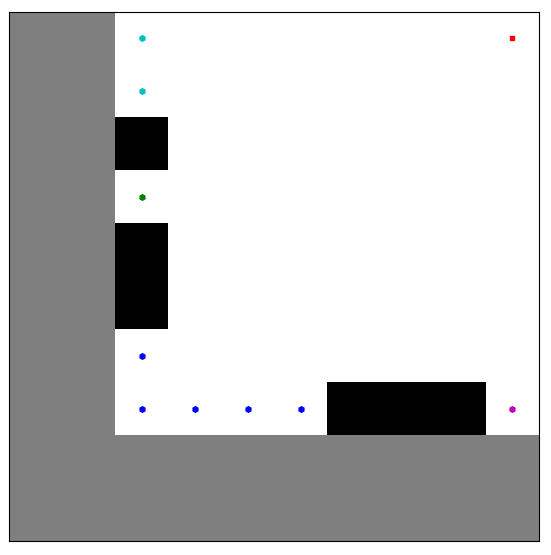
\includegraphics[width=0.5\textwidth]{frontiers.png}
    \label{fig:frontiers}
    \caption{frontiers}
\end{figure}
\FloatBarrier

\section{Build the path}

\section{Follow the path}

